% arara: pdflatex
% arara: biber
% arara: pdflatex
% arara: pdflatex

\documentclass{article}

\usepackage{beamerarticle}
\usetheme{CambridgeUS}
\usecolortheme{crane}
\usepackage[
  backend=biber,
  style=authoryear-comp,
  useprefix=false,
  sorting=ynt
]{biblatex}

\usepackage{subfiles}
\usepackage{stmaryrd}
\usepackage[]{amsmath}
\usepackage{amsfonts}
\usepackage{amssymb}
\usepackage{mathtools}
\usepackage{forest}
\usepackage{tabularx}
\usepackage{linguex}
\usepackage{centernot}
\usepackage{todonotes}
\useforestlibrary{linguistics}

\tikzset{
    invisible/.style={opacity=0,text opacity=0},
    visible on/.style={alt=#1{}{invisible}},
    alt/.code args={<#1>#2#3}{%
      \alt<#1>{\pgfkeysalso{#2}}{\pgfkeysalso{#3}} % \pgfkeysalso doesn't change the path
    },
}
\forestset{
  visible on/.style={
    for current and ancestors={
      /tikz/visible on={#1},
      edge={/tikz/visible on={#1}}}}}

\forestset{tree defaults/.style={for tree={parent anchor=south, child anchor=north},every tree node/.style={align=center,anchor=north},level/.style={sibling distance=50mm/#1},baseline}}

\forestset{en/.style={parent anchor=center, child anchor=center}}
\forestset{em/.style={parent anchor=north west, child anchor=north west}}
\forestset{el/.style={parent anchor=north, child anchor=north}}

\usetikzlibrary{positioning}
\usetikzlibrary{calc}
\usetikzlibrary{arrows}
\usetikzlibrary{decorations.markings}
%\DeclareNameFormat{labelname:poss}{% Based on labelname from biblatex.def
%  \ifcase\value{uniquename}%
%  \usebibmacro{name:last}{#1}{#3}{#5}{#7}%
%  \or
%  \ifuseprefix
%  {\usebibmacro{name:first-last}{#1}{#4}{#5}{#8}}
%  {\usebibmacro{name:first-last}{#1}{#4}{#6}{#8}}%
%  \or
%  \usebibmacro{name:first-last}{#1}{#3}{#5}{#7}%
%  \fi
%  \usebibmacro{name:andothers}%
%  \ifnumequal{\value{listcount}}{\value{liststop}}{'s}{}
%}
%
%\DeclareFieldFormat{shorthand:poss}{%
%  \ifnameundef{labelname}{#1's}{#1}
%}
%
%\DeclareFieldFormat{citetitle:poss}{\mkbibemph{#1}'s}
%
%\DeclareFieldFormat{label:poss}{#1's}
%
%\newrobustcmd*{\posscitealias}{%
%  \AtNextCite{%
%    \DeclareNameAlias{labelname}{labelname:poss}%
%    \DeclareFieldAlias{shorthand}{shorthand:poss}%
%    \DeclareFieldAlias{citetitle}{citetitle:poss}%
%    \DeclareFieldAlias{label}{label:poss}
%  }
%}
%
%\newrobustcmd*{\posscite}{%
%  \posscitealias%
%  \textcite
%}
%
%\newrobustcmd*{\Posscite}{\bibsentence\posscite}
%
%\newrobustcmd*{\posscites}{%
%  \posscitealias%
%  \textcites
%}

\newcommand\quelle[1]{{%
  \unskip\nobreak\hfil\penalty50
  \hskip2em\hbox{}\nobreak\hfil#1%
  \parfillskip=0pt \finalhyphendemerits=0 \par
}
}

\newcommand{\figex}{\refstepcounter{ExNo}\theExNo\hspace{\Exlabelsep}}

\newcounter{DerivStep}

\newcommand{\hxp}{$\left\{ \text{X, YP} \right\}$}
\newcommand{\hh}{$\left\{ \text{X, Y} \right\}$}
\newcommand{\xpyp}{$\left\{ \text{XP, YP} \right\}$}
\bibliography{Thesis}
%\AtBeginSection[]
%{
%  \begin{frame}
%    \frametitle{Table of Contents}
%    \tableofcontents[currentsection]
%  \end{frame}
%}
\title{Explaining the Resultative Parameter}
\subtitle{Thesis Proposal}
\author{Dan Milway}
\AtBeginSection[]{
  \begin{frame}
  \vfill
  \centering
  \begin{beamercolorbox}[sep=8pt,center,shadow=true,rounded=true]{title}
    \usebeamerfont{title}\insertsectionhead\par%
  \end{beamercolorbox}
  \vfill
  \end{frame}
}

\begin{document}
\section{}
\frame[plain]{\titlepage}
\section[What is the Resultative Parameter?]{What is the Resultative Parameter?}
\begin{frame}
  \frametitle{What is the resultative parameter?}
  \begin{itemize}
    \item Resultative interpretation of secondary predicates
      \begin{itemize}
	\item<1-> Some languages allow it (\textit{e.g.} Germanic languages)
	\item<4-> Some disallow it (\textit{e.g.} Romance Languages)
      \end{itemize}
  \end{itemize}
  \begin{overprint}
    \onslide<2>
    \ex. English
    \a. I ate the fish raw. (depictive)
    \b. I hammered the metal flat. (resultative)
    \z.

    \onslide<3>
    \ex.German 
    \ag. Er i\ss{}t das Fleisch roh.\\
    He eats the meat raw\\
    ``He's eating the meat raw.'' (depictive)\\
    \parencite{muller2004analysis}
    \bg. Wir haben die teekanne leer getrunken.\\
    we have the teapot empty drink.\textsc{part}\\
    ``We drank the teapot dry.''(resultative)\\
    \parencite{kratzer_building_2004}
    \z.

    \onslide<5>
    \ex. French
    \ag. Pierre mange la viande crue.\\
    Pierre eat.3sg the.fem meat raw.fem\\
    ``Pierre ate the meat raw'' (depictive)\\
    \parencite{legendre1997secondary}
    \bg.* Il a march\'e les jambes raides.\\
    He has walked the legs stiff\\
    ``He walked his legs off.'' (resultative)\\
    \parencite{washio1997resultatives}
    \z.

    \onslide<6>
    \ex. Italian
    \ag. l' ho mangiato crudo.\\
    3sg \textsc{aux}.1sg eaten raw\\
    ``I ate it raw'' (depictive)
    \bg.* l' ho bevuto vuoto.\\
    3sg \textsc{aux}.1sg drank empty\\
    ``I drank it dry'' (resultative)
    \z.

  \end{overprint}
\end{frame}
\begin{frame}
  \frametitle{Why does it need to be explained?}
  \begin{itemize}
    \item It's not directly learnable from the PLD.
      \begin{itemize}
	\item<3-> Compare this to V-to-T movement.
      \end{itemize}
  \end{itemize}
  \begin{overprint}
    \onslide<2>
    \ex. English-type (SP)
    \a. \textsc{Subj} V \textsc{Obj} Adj (depictive)
    \b. \textsc{Subj} V \textsc{Obj} Adj (resultative)

    \ex. French-type (SP)
    \a. \textsc{Subj} V \textsc{Obj} Adj (depictive)
    \b.* \textsc{Subj} V \textsc{Obj} Adj (resultative)

    \onslide<3>
    \ex. English-type (Y/N)
    \a. \textsc{do Subj} V \textsc{Obj}? 
    \b.* V \textsc{Subj} \textsc{Obj}?

    \ex. German-type (Y/N)
    \a.* \textsc{do Subj} V \textsc{Obj}? 
    \b. V \textsc{Subj} \textsc{Obj}?

    \onslide<4>
    \begin{figure}[h]
      \centering
      \begin{tikzpicture}
	\node (param) at (0,0) {\{*\}V-to-T};
	\node (PLD) at (4,0) {PLD};
	\node (UG) at (0,-2) {UG};
	\draw[->] (PLD) -- (param);
	\draw[->] (UG) -- (param);
      \end{tikzpicture}
      \caption{Acquiring V-to-T}
      \label{fig:VtoTAcq}
    \end{figure}
    \onslide<5>
    \begin{figure}[h]
      \centering
      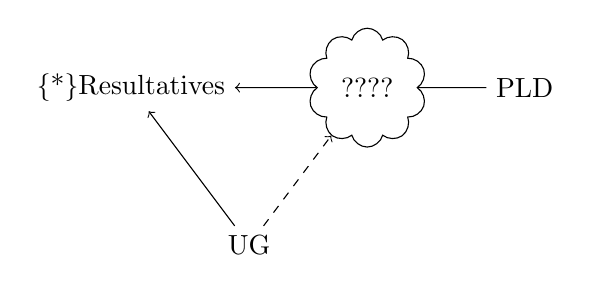
\begin{tikzpicture}
	\node (param) at (0,0) {\{*\}Resultatives};
	\node[cloud,draw] (cloud) at (3,0) {????};
	\node (PLD) at (5,0) {PLD};
	\node (UG) at (1.5,-2) {UG};
	\draw (PLD) -- (cloud);
	\draw[->] (cloud) -- (param);
	\draw[->] (UG) -- (param);
	\draw[->,dashed] (UG) -- (cloud);
      \end{tikzpicture}
      \caption{Acquiring Resultatives}
      \label{fig:resAcq}
    \end{figure}
  \end{overprint}
\end{frame}
\begin{frame}
  \begin{block}
    {My Thesis Project:}
    \begin{itemize}
      \item Explaining how a semantic ``parameter setting'' can be acquired from surface phenomena in the PLD.
    \end{itemize}
    \onslide<2>{
      In other words:
    \begin{itemize}
      \item Figuring out what's behind those question marks.
    \end{itemize}}
  \end{block}
  \onslide<2>{
      \centering
      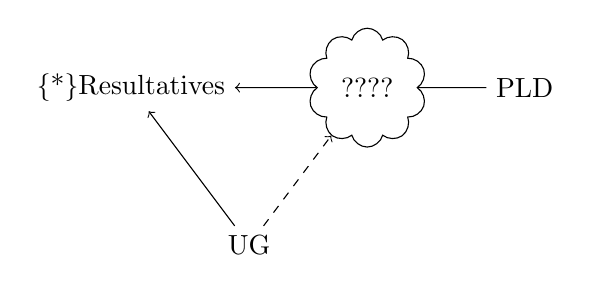
\begin{tikzpicture}
	\node (param) at (0,0) {\{*\}Resultatives};
	\node[cloud,draw] (cloud) at (3,0) {????};
	\node (PLD) at (5,0) {PLD};
	\node (UG) at (1.5,-2) {UG};
	\draw (PLD) -- (cloud);
	\draw[->] (cloud) -- (param);
	\draw[->] (UG) -- (param);
	\draw[->,dashed] (UG) -- (cloud);
      \end{tikzpicture}
  }
\end{frame}
\section{How will I explain it?}
\begin{frame}
  \frametitle{Ingredients of an explanation}
  \begin{enumerate}
    \item A structural analysis of resultatives.
    \item The surface phenomena associated with \{*\}Resultatives.
    \item A way of linking the first two ingredients.
  \end{enumerate}
\end{frame}
\begin{frame}
  \frametitle{Ingredients of an explanation}
  \begin{enumerate}
    \setcounter{enumi}{0}
    \item A structural analysis of resultatives.
  \end{enumerate}
  {\rm Natalie hammered the metal flat.}\\
  {\footnotesize
  \begin{forest}
    nice empty nodes,sn edges,baseline,for tree={
    calign=fixed edge angles,
  calign primary angle=-30,calign secondary angle=70}
    [AgrOP
      [DP,[{\rm the metal},roof,name=obj]]
      [
	[AgrO]
	[VP
	  [VP,calign=center
	    [{\rm hammer}]
	    [$\langle$DP$\rangle$,name=theme]
	  ]
	  [resP
	    [$\langle$DP$\rangle$,name=spec res]
	    [
	      [res]
	      [SC
		[$\langle$DP$\rangle$,name=SC theme]
		[{\rm flat}]
	      ]
	    ]
	  ]
	]
      ]
    ]
    \draw[->] (SC theme) to[out=west, in=south] (spec res);
    \draw[->] (spec res) to[out=south, in=south] (theme);
    \draw[->] (theme) to[out=south west, in=south] (obj);
  \end{forest}}
\end{frame}
\begin{frame}
  \frametitle{Ingredients of an explanation}
  \begin{enumerate}
    \setcounter{enumi}{1}      
    \item The surface phenomena associated with \{*\}Resultatives.
      \begin{itemize}
	\item What learnable pattern correlates with resultatives?
        \item Resultatives are strongly correlated with Productive Bare-Stem Compounding. \parencite[][and following]{snyder1995language}
	\item I propose that Bare-Stem Compounding is allowed iff a language's lexicon has Bare Stems.
      \end{itemize}
  \end{enumerate}
\end{frame}
\begin{frame}
  \frametitle{Ingredients of an explanation}
  \begin{enumerate}
    \setcounter{enumi}{2}  
    \item A way of linking the first two ingredients.
      \begin{itemize}
	\item A modified version of Chomsky's (\citeyear{chomsky2013problems,chomsky2015problems}) Label Theory
	\item Resultative SP is derivable only if the secondary predicate is instantiated by a bare stem.
      \end{itemize}
  \end{enumerate}
\end{frame}
\section{What are resultatives?}
\begin{frame}
  \frametitle{Interpretive properties}
  \ex.
  \a. {\rm Natalie hammered the metal flat.}
  \b. There was a hammering event $e$, Natalie was the agent of $e$, and \alert<2>{the metal} was the theme of $e$.\\
  $e$ \alert<3>{caused} a flatness state $s$, and \alert<2>{the metal} was the theme of $s$.

  \pause
  \begin{enumerate}
    \item \alert<2>{Argument Sharing}
    \item \alert<3>{Causativity}
  \end{enumerate}
\end{frame}
\subsection{Argument Sharing}
\begin{frame}
  \frametitle{What is Argument Sharing?}
  When a single object/element/phrase/symbol/\textit{etc.} is an argument of multiple predicates.
\end{frame}
\begin{frame}
  \frametitle{Non-resultative Argument Sharing}
  \pause
  \ex. \textbf{Control}\\
    {\rm Alice wants to win.}\\
    Alice$_i$ wants [$ec_i$ to win]

  \pause
\ex. \textbf{Parasitic Gaps}\\
    {\rm Who did you discuss without meeting?}\\
    Who$_i$ did you [[discuss $ec_i$] [without meeting $ec_i$]]?
    
    \pause
    \ex. \textbf{Depictives}\\
    {\rm Monica left angry.}\\
    Monica$_i$ left [$ec_i$ angry].

\end{frame}
\begin{frame}
  {What does Argument Sharing look like?}
  \begin{itemize}
    \item Where are the shared arguments?
    \item What are those $ec$s?
  \end{itemize}
  
\end{frame}
\subfile{UTAH}
\subfile{MTC}
\begin{frame}
  \frametitle{Deriving Resultatives}
  \ex.{\rm Natalie hammered the metal flat.}

  \begin{columns}
    \begin{column}[T]{0.5\textwidth}
      \begin{block}
	{Build the adjunct}
	\begin{itemize}
	  \item<2-> Build the Small Clause
	  \item<3-> Merge(\textit{res}$^\circ$, $\alpha$)
	  \item<4-> Copy(DP) + Merge(DP, $\beta$)
	  \item<5-> Copy(DP)
	\end{itemize}
      \end{block}
    \only<5->{
      \begin{forest}
	[DP[{\rm the metal},roof]]
      \end{forest}}
    \end{column}
    \begin{column}[T]{0.5\textwidth}
      {\small
      \begin{forest}
	nice empty nodes,sn edges,baseline
	[$\gamma$,visible on=<4-5>
	  [DP,visible on=<4-5> [{\rm the metal},roof,visible on=<4-5>]]
	  [$\beta$,visible on=<4-5>
	    [\textit{res},visible on=<3-5>]
	    [$\alpha$,visible on=<3-5>
	      [DP [{\rm the metal},roof,visible on=<2-5>]]
	      [{\rm flat},visible on=<2-5>]
	    ]
	  ]
	]
      \end{forest}
    }
    \end{column}
  \end{columns}
\end{frame}
\begin{frame}
  \frametitle{Deriving Resultatives}
  \ex.{\rm Natalie hammered the metal flat.}

  \begin{columns}
    \begin{column}[T]{0.5\textwidth}
      \begin{block}
	{Build the VP}
	\begin{itemize}
	  \item<2-> Merge({\rm hammer}, DP) 
	  \item<3-> Merge($\delta$, $\gamma$)
	  \item<4-> \dots
	\end{itemize}
      \end{block}
    \only<1>{
      \begin{forest}
	[DP[{\rm the metal},roof]]
      \end{forest}}
    \end{column}
    \begin{column}[T]{0.5\textwidth}
    {\small
      \begin{forest}
	nice empty nodes,sn edges,baseline
	[$\zeta$,visible on=<3->
	  [$\delta$,visible on=<3->
	    [{\rm hammer},visible on=<2->]
	    [DP,visible on=<2-> [{\rm the metal},visible on=<2->]]
	  ]
	  [$\gamma$,visible on=<3->]
	]
      \end{forest}
    }
    \end{column}
  \end{columns}
\end{frame}

\section{Label Theory}
\begin{frame}
  {Label Theory}
  {\textcite{chomsky2013problems,chomsky2015problems}}
  \begin{itemize}
    \item UG is reducible to simplest merge
  \end{itemize}
  \ex. Merge($\alpha,\beta$) = $\left\{ \alpha,\beta \right\}$

  \begin{itemize}
    \item Accounts for the fundamental properties of language (\textit{e.g.}, structure-dependence of rules, displacement)
      \begin{itemize}
	\item Except for Projection/Labeling
      \end{itemize}
    \item Chomsky's proposal: Labels are assigned at the CI interface by a Labeling Algorithm (LA)
  \end{itemize}
\end{frame}
\begin{frame}
  {The Labeling Algorithm}
  \begin{itemize}
    \item LA is a special instance of Minimal Search.
      \begin{itemize}
	\item Picks out the most prominent item as a syntactic object's label
      \end{itemize}
      \pause
    \item There are three relevant classes of syntactic objects for LA:
  \end{itemize}
  \begin{overprint}
    \onslide<3>
    \begin{block}
      {(i) Head-Phrase Structures}
      \begin{itemize}
	\item Label($\left\{ \text{X, YP} \right\}$) = X
      \end{itemize}
    \end{block}
    \onslide<4-5>
    \begin{block}
      {(ii) Head-Head Structures}
      \begin{itemize}
	\item<4-5> Label($\left\{ \text{X, }\textsc{root} \right\}$) = X
	  \begin{itemize}
	    \item<4-5> Roots cannot label
	  \end{itemize}
	\item<5> Undefined otherwise
      \end{itemize}
    \end{block}
    \onslide<6-8>
    \begin{block}
      {(iii) Phrase-Phrase Structures}
      \begin{itemize}
	\item<6-8> Label($\left\{ \text{XP}, \langle\text{YP}\rangle \right\}$) = Label(XP)
	  \begin{itemize}
	    \item<6-8> Lower copies are invisible to LA.
	  \end{itemize}
	\item<7-8> Label($\left\{ \text{XP}_F, \text{YP}_F \right\}$)= $\langle\text{F,F}\rangle$
	  \begin{itemize}
	    \item<7-8> Iff XP and YP agree for some feature F
	  \end{itemize}
	\item <8> Undefined otherwise
      \end{itemize}
    \end{block}
  \end{overprint}
\end{frame}
\begin{frame}
  {My extensions to Label Theory}
  \begin{block}
    {Labels determine composition}
    \begin{itemize}
      \item<2-> If Label(SO) $\in$ SO, then SO composes by function application
	\begin{itemize}
	  \item<3-> $\llbracket\left\{ \text{X, YP} \right\}\rrbracket$ = X(YP)
	\end{itemize}
      \item<4-> If Label(SO) = $\langle\text{F,F}\rangle$, then SO is interpreted as an Operator-variable structure
	\begin{itemize}
	  \item<5-> $\llbracket\left\{ \text{DP}_Q, \text{CP}_Q \right\}\rrbracket$ = $(\text{Wh}x)(\dots x \dots)$
	\end{itemize}
    \end{itemize}
  \end{block}
\end{frame}
\begin{frame}
  {My extensions to Label Theory}
  \begin{block}
    {Adjunction structures are unlabeled}
    \begin{itemize}
      \item Adjuncts are ignored by LA.
	\begin{itemize}
	  \item Label($\left\{ \text{XP, ZP} \right\}$) = $\emptyset$ if ZP is an adjunct
	  \item Since ZP is ignored by LA, it is internally unlabelled. (Label(ZP)=$\emptyset$)
	\end{itemize}
	\pause
      \item Unlabeled SOs compose by conjuction.
	\begin{itemize}
	  \item $\llbracket\left\{ \text{XP, ZP} \right\}\rrbracket$ = XP \& ZP (if $\left\{ \text{XP, ZP} \right\}$ is unlabelled)
	\end{itemize}
    \end{itemize}
  \end{block}
\end{frame}
\begin{frame}
  {What can this version of Label Theory get us?}
  \begin{block}
    {Subjects of ACC-ing clauses and pseudo-relatives}
    \begin{itemize}
      \item<2-> \textcite{cinque1996pseudo} shows that the position of an ACC-ing/pseudo-relative clause affects the behaviour of its subject.
    \end{itemize}
    \only<2->{
    \ex. \textbf{Italian pseudo-relative (PR)}\\
    {\rm Mario che correva a tutti velocit\`a}

    \ex. \textbf{English ACC-ing clause (AC)}\\
    {\rm Mario running at full speed}

  }
    \begin{itemize}
      \item<3-> If the AC/PR is a complement of V, the subject cannot move.
      \item<3-> If the AC/PR is a VP adjunct, the subject must move.
    \end{itemize}
  \end{block}
\end{frame}
\begin{frame}
  {What can this version of Label Theory get us?}

    \begin{columns}
    \begin{column}[T]{0.6\textwidth}
      {\rm *Mario$_i$ was [$_{VP}$ [seen[$t_i$ running]]]}
      \begin{block}
	{Complement ACs}
	\begin{itemize}
	  \item Subject is frozen in the AC
	  \item Prog$^\circ$ is too weak to label $\zeta$
	    \begin{itemize}
	      \item Compare Chomsky's (2015) discussion of EPP
	    \end{itemize}
	  \item If {\rm Mario} were \textit{in situ}, Label($\zeta$) = $\langle\text{F,F}\rangle$
	  \item Lower copies are invisible, so $\zeta$ is unabelable.
	  \item The derivation crashes at CI
	\end{itemize}
      \end{block}
    \end{column}
    \begin{column}[T]{0.4\textwidth}
	{\small
	  \begin{forest}
	    nice empty nodes,sn edges,baseline
	    [$\alpha$
	      [{\rm Mario}]
	      [$\beta$
		[T]
		[$\gamma$
		  [Voice$_{pass}$]
		  [$\delta$
		    [{\rm see}]
		    [$\zeta$
		      [$\langle${\rm Mario}$\rangle$]
		      [Prog]
		    ]
		  ]
		]
	      ]
	    ]
	  \end{forest}
	}
    \end{column}
  \end{columns}
\end{frame}
\begin{frame}
  {What can this version of Label Theory get us?}
  \begin{columns}
    \begin{column}[T]{0.55\textwidth}
      {\rm *I [ [$_{VP}$ saw Bill] [Mario running]]}
      \begin{block}
	{Adjunct ACs}
	\begin{itemize}
	  \item Subjects must move to theme position
	  \item $\eta$ is adjoined, therefore ignored by LA
	  \item $\eta$ is interpreted as the conjunction of {\rm Mario} and {\rm running}
	    \begin{itemize}
	      \item This is an ill-formed interpretation
	    \end{itemize}
	\end{itemize}
      \end{block}
    \end{column}
    \begin{column}[T]{0.45\textwidth}
      {\small
	  \begin{forest}
	    nice empty nodes,sn edges,baseline
	    [$\alpha$
	      [{\rm I}]
	      [$\beta$
		[Voice]
		[$\gamma$
		  [$\zeta$
		    [{\rm see}]
		    [{\rm Bill}]
		  ]
		  [$\eta$
		    [{\rm Mario}]
		    [Prog]
		  ]
		]
	      ]
	    ]
	  \end{forest}
	}
    \end{column}
  \end{columns}
\end{frame}
\begin{frame}
  {What can this version of Label Theory get us?}
    
\end{frame}
\section{Deriving the Resultative Parameter}
\begin{frame}
  {Recapping Resultatives and Compounding}

  {\rm Natalie hammered the metal flat.}
  {\small
  \begin{forest}
    nice empty nodes,sn edges,baseline,for tree={
    calign=fixed edge angles,
  calign primary angle=-30,calign secondary angle=70}
    [$\kappa$
      [DP,[{\rm the metal},roof,name=obj]]
      [$\eta$
	[AgrO]
	[$\zeta$,calign=fixed edge angles,calign primary angle=-30,calign secondary angle=70
	  [$\delta$
	    [{\rm hammer}]
	    [$\langle$DP$\rangle$,name=theme]
	  ]
	  [$\gamma$,calign=fixed edge angles,calign primary angle=-30,calign secondary angle=70
	    [$\langle$DP$\rangle$,name=spec res]
	    [$\beta$
	      [res]
	      [$\alpha$
		[$\langle$DP$\rangle$,name=SC theme]
		[{\rm flat}]
	      ]
	    ]
	  ]
	]
      ]
    ]
    \draw[->] (SC theme) to[out=west, in=south] (spec res);
    \draw[->] (spec res) to[out=south, in=south] (theme);
    \draw[->] (theme) to[out=south west, in=south] (obj);
  \end{forest}}
\end{frame}
\begin{frame}
  {Recapping Resultatives and Compounding}
  \begin{block}
    {The Compounding Parameter}
    \begin{itemize}
      \item $\left\{ \text{*} \right\}$Resultatives is linked to $\left\{ \text{*} \right\}$bare-stem compounding.
      \item Bare-stem compounding requires bare stems.
      \item Bare stems require category heads without $\varphi$-features ($n_\emptyset$, $adj_\emptyset$, \textit{etc}).
      \item English-type languages have $adj_\emptyset$ (and maybe $adj_\varphi$).
      \item French-type languages have only $adj_\varphi$
    \end{itemize}
  \end{block}
\end{frame}
\begin{frame}
  So now let's show:
  \begin{enumerate}
    \item<2-> Resultatives can be derived with $adj_\emptyset$
    \item<3> Resultatives cannot be derived with $adj_\varphi$
  \end{enumerate}
\end{frame}
\begin{frame}
  {English-type languages: \checkmark Resultatives}

  {\rm hammer the metal flat}
  \begin{columns}
    \begin{column}[T]{0.5\textwidth}
      \begin{block}
	{Deriving the adjunct}
	\begin{itemize}
	  \item<2-> Build the Small Clause.
	  \item<3-> Merge(res, $\beta$)
	  \item<4-> Copy(DP) + Merge(DP, $\gamma$)
	  \item<6-> Transfer($\beta$)
	    \begin{itemize}
	      \item res is a phase head.
	      \item Label($\beta$) = Label($\alpha$)
	      \item $\beta$ converges.
	    \end{itemize}
	  \item<7-> Copy(DP)
	\end{itemize}
      \end{block}
      \only<7->{\small
	\begin{forest}
	  nice empty nodes,sn edges,baseline
	  [DP$_\varphi$[{\rm the metal},roof]]
	\end{forest}
      }
      \only<4-5>{\small
	\begin{forest}
	  nice empty nodes,sn edges,baseline
	  [DP$_\varphi$[{\rm the metal},roof]]
	\end{forest}
      }
    \end{column}
    \begin{column}[T]{0.5\textwidth}
      {\small
	\begin{forest}
	  nice empty nodes,sn edges,baseline,for tree={
	  calign=fixed edge angles,
	  calign primary angle=-30,calign secondary angle=50}
	  [$\delta$,visible on=<5->
	    [DP$_\varphi$,visible on=<5->[{\rm the metal},roof,visible on=<5->]]
	    [$\gamma$,visible on=<5->
	      [res,visible on=<3->]
	      [$\beta$,visible on=<3->
		[DP$_\varphi$,visible on=<2->[{\rm the metal},name=SC DP,roof,visible on=<2->]]
		[$\alpha$,visible on=<2->
		  [adj$_\emptyset$,visible on=<2->]
		  [{\rm flat},visible on=<2->]
		]
	      ]
	    ]
	  ]
	  \only<6->{
	  \draw[thick] ([xshift=-36pt, yshift=-24pt]SC DP) arc[start angle=170,end angle=130,radius=7.5cm];
	}
	\end{forest}
      }
    \end{column}
  \end{columns}
\end{frame}
\begin{frame}
  {English-type languages: \checkmark Resultatives}

  {\rm hammer the metal flat}
  \begin{columns}
    \begin{column}[T]{0.5\textwidth}
      \begin{block}
	{Deriving the VP}
	\begin{itemize}
	  \item<2-> Merge(DP, {\rm hammer})
	  \item<3-> Merge($\zeta$, $\delta$)
	  \item<4-> Merge(AgrO, $\eta$)
	  \item<5-> Copy(DP) + Merge(DP, $\kappa$)
	  \item<6-> \ldots
	\end{itemize}
      \end{block}
      \only<1-3>{\small
	\begin{forest}
	  nice empty nodes,sn edges,baseline
	  [$\delta$
	    [DP$_\varphi$]
	    [$\gamma$
	      [res]
	      [($\beta$]
	    ]
	  ]
	\end{forest}
      }
      \only<1-2>{\small
	\begin{forest}
	  nice empty nodes,sn edges,baseline
	  [DP$_\varphi$[{\rm the metal},roof]]
	\end{forest}
      }
    \end{column}
    \begin{column}[T]{0.5\textwidth}
      {\small
	\begin{forest}
	  nice empty nodes,sn edges,baseline,for tree={
    calign=fixed edge angles,
  calign primary angle=-30,calign secondary angle=50}
	  [$\mu$,visible on=<5->
	    [DP$_\varphi$,visible on=<5->[{\rm the metal},roof,visible on=<5->]]
	    [$\kappa$,visible on=<5->
	      [AgrO$_\varphi$,visible on=<4->]
	      [$\eta$,visible on=<4->
		[$\zeta$,visible on=<3->
		  [DP$_\varphi$,visible on=<2->[{\rm the metal},roof,visible on=<2->]]
		  [{\rm hammer},visible on=<2->]
		]
		[$\delta$\\\ldots,align=center,visible on=<3->
		  %[DP$_\varphi$[{\rm the metal},roof]]
		  %[$\gamma$
		  %  [res]
		  %  [$\beta$]
		  ]
		]
	      ]
	    ]
	\end{forest}
      }
    \end{column}
  \end{columns}
\end{frame}
\begin{frame}
  So now let's show:
  \begin{enumerate}
    \item Resultatives can be derived with $adj_\emptyset$
      \begin{itemize}
	\item \alert{Shown}
      \end{itemize}
    \item Resultatives cannot be derived with $adj_\varphi$
  \end{enumerate}
\end{frame}
\begin{frame}
  {French-type languages: *Resultatives}
  {Derivation Attempt 1: Just like English-type}

  {\rm *marcher les jambes raides}
  \begin{columns}
    \begin{column}[T]{0.5\textwidth}
      \begin{block}
	{Deriving the adjunct}
	\begin{itemize}
	  \item<2-> Build the Small Clause.
	  \item<3-> Merge(res, $\beta$)
	  \item<4-> Copy(DP) + Merge(DP, $\gamma$)
	  \item<6-> Transfer($\beta$)
	    \begin{itemize}
	      \item res is a phase head.
	      \item Lower DP copy is invisible
	      \item adj$_\varphi$ is too weak to label without agreement
	      \item Label($\beta$) is undefined
	      \item *CRASH*
	    \end{itemize}
	\end{itemize}
      \end{block}
    \end{column}
    \begin{column}[T]{0.5\textwidth}
      {\small
	\begin{forest}
	  nice empty nodes,sn edges,baseline,for tree={
	  calign=fixed edge angles,
	  calign primary angle=-30,calign secondary angle=50}
	  [$\delta$,visible on=<5->
	    [DP$_\varphi$,visible on=<5->[{\rm les jambes},roof,visible on=<5->]]
	    [$\gamma$,visible on=<5->
	      [res,visible on=<3->]
	      [$\beta$,visible on=<3->
		[DP$_\varphi$,visible on=<2->[{\rm les jambes},name=SC DP,roof,visible on=<2->]]
		[$\alpha$,visible on=<2->
		  [adj$_\varphi$,visible on=<2->]
		  [{\rm raides},visible on=<2->]
		]
	      ]
	    ]
	  ]
	  \only<6->{
	  \draw[thick] ([xshift=-36pt, yshift=-24pt]SC DP) arc[start angle=170,end angle=130,radius=7.5cm];
	}
	\end{forest}
      }
    \end{column}
  \end{columns}
\end{frame}
\begin{frame}
  So now let's show:
  \begin{enumerate}
    \item Resultatives can be derived with $adj_\emptyset$
      \begin{itemize}
	\item Shown
      \end{itemize}
    \item Resultatives cannot be derived with $adj_\varphi$
      \begin{itemize}
	\item \alert{Not shown yet}
      \end{itemize}
  \end{enumerate}
\end{frame}
\begin{frame}
  {French-type languages: *Resultatives}
  {Derivation Attempt 2}

  \begin{columns}
    \begin{column}[T]{0.5\textwidth}
      {\rm *marcher les jambes raides}
      \begin{block}
	{Deriving the adjunct}
	\begin{itemize}
	  \item <2-> Build the Small Clause.
	  \item <3-> Merge(res, $\beta$)
	  \item <4-> Transfer($\beta$)
	    \begin{itemize}
	      \item res is a phase head.
	      \item DP and $\alpha$ agree for $\varphi$.
	      \item Label($\beta$)= $\langle\varphi,\varphi\rangle$
	      \item $\beta$ converges.
	    \end{itemize}
	\end{itemize}
      \end{block}
    \end{column}
    \begin{column}[T]{0.5\textwidth}
      {\small
	\begin{forest}
	  nice empty nodes,sn edges,baseline,for tree={
	  calign=fixed edge angles,
	  calign primary angle=-30,calign secondary angle=50}
	    [$\gamma$,visible on=<3->
	      [res,visible on=<3->]
	      [$\beta$,visible on=<3->
		[DP$_\varphi$,visible on=<2->[{\rm les jambes},name=SC DP,roof,visible on=<2->]]
		[$\alpha$,visible on=<2->
		  [adj$_\varphi$,visible on=<2->]
		  [{\rm raides},visible on=<2->]
		]
	      ]
	    ]
	  \only<4->{
	  \draw[thick] ([xshift=-36pt, yshift=-24pt]SC DP) arc[start angle=170,end angle=130,radius=7.5cm];
	}
	\end{forest}
      }
    \end{column}
  \end{columns}
\end{frame}
\begin{frame}
  {French-type languages: *Resultatives}
  {Derivation Attempt 2}
  \begin{columns}
    \begin{column}[T]{0.5\textwidth}
      {\rm *marcher les jambes raides}
      \begin{block}
	{Deriving the VP}
	\begin{itemize}
	  \item<2-> Merge({\rm march-}, DP)
	    \begin{itemize}
	      \item<3-> DP is unavailable
	      \item<4->  *CRASH*
	    \end{itemize}
	\end{itemize}
      \end{block}
      {\small
	\begin{forest}
	  nice empty nodes,sn edges,baseline
	    [$\gamma$
	      [res]
	      [($\beta$]
	    ]
	\end{forest}
      }
    \end{column}
    \begin{column}[T]{0.5\textwidth}
      \begin{forest}
	[*,visible on=<4->
	  [{\rm march-},visible on=<2->]
	  [DP$_\varphi$,visible on=<2->]
	]
      \end{forest}
    \end{column}
  \end{columns}
\end{frame}
\begin{frame}
  So now let's show:
  \begin{enumerate}
    \item Resultatives can be derived with $adj_\emptyset$
      \begin{itemize}
	\item Shown
      \end{itemize}
    \item Resultatives cannot be derived with $adj_\varphi$
      \begin{itemize}
	\item \alert{Shown}\footnote{I think}
      \end{itemize}
  \end{enumerate}
\end{frame}
\end{document}
